\section{RGB Identification with Solver-Driven Gaussians}
\label{sec:solver-driven}
\raggedbottom
This qualification closes a different connection from the soft-constrained PIDG hybrid: rendered Gaussian motion is generated by integrated mechanics. We infer physical coefficients from an observed RGB prefix, freeze them, and forecast changed controls and contact without a temporal deformation network or future-frame fitting. The experiment supplies initial volume, appearance, density, cameras and floor geometry; it does not establish automatic volumetric reconstruction from arbitrary video.

\paragraph{Representation and observation model.}
A $120\times60\times60$\,mm block has 225 nodes and 768 tetrahedra. Its 10,059 retained appearance Gaussians bind to containing tetrahedra. For reference center $\mu_i^0$, shape weights $N_{ia}$ and nodal displacement $u_a$, transport is
\begin{equation}
 \mu_i(t)=\mu_i^0+\sum_a N_{ia}u_a(t),\quad
 F_i=I+\sum_a u_a\otimes\nabla N_{ia},\quad
 \Sigma_i(t)=F_i\Sigma_i^0 F_i^\top.
\end{equation}
Polar rotation transports spherical-harmonic viewing directions into the material frame. Displacement-form transport preserves the initial render exactly. Surface splats outside the supplied block (36.79\% of retained centers) use explicit affine extension; their centers are not interpreted as occupied material. Appearance remains fixed throughout this qualification.

\paragraph{Mechanics and Gaussian boundary coefficients.}
The frozen learned invariant-energy decoder supplies stress, with one fitted positive material scale and a fixed material-family descriptor. Eight candidate Gaussian attachment patches lie on the two end faces. Their nonnegative stiffness coefficients, one moving Gaussian target stiffness, and a mass-proportional damping rate are fitted with the material scale (11 coefficients). Gaussian integrals use lumped-volume quadrature, and floor contact uses surface-area quadrature. Gravity, density $625$\,kg/m$^3$, prescribed target paths, and release times are supplied. The moving target is a compliant distributed interaction, not a unilateral rigid poker. Symplectic Euler integrates the dynamics at $0.1$\,ms for forecasting. Floor and reciprocal two-body contact use finite penalties; this experiment includes neither friction nor continuous collision detection.

\paragraph{Calibration and controls.}
An independent analytic Mooney--Rivlin model generates the numerical reference. Only images from the first $0.14$\,s in two cameras are available for fitting; two other cameras are withheld. The 144 prefix images include reserved calibration validation images. No material, force, interior-position or future-image labels enter the successful RGB fit. A generic 54-proposal bank spans material scale, either support face, total attachment stiffness and target stiffness. Fitting-image RGB scores initialize 80 differentiable rollout updates; reserved foreground PSNR selects the checkpoint. The matched analytic control replaces the frozen learned law with neo-Hookean energy and receives the same bank and refinement budgets. Calibration is iterative; subsequent prediction uses frozen coefficients and forward integration only.

A separate diagnostic first reconstructs nodal motion from images and then solves linear inverse dynamics. Despite good image fits, its unobserved interior accelerations are unsuitable for force identification, and the resulting calibration scores are approximately 20\,dB. The proposal-bank initialization avoids this failure. Reserved foreground PSNR reaches 52.01\,dB for solver-driven learned mechanics and 48.77\,dB for the analytic control. Fixed-appearance temporal-network adaptations reach 37.07\,dB (released PIDG deformation/TV architecture) and 38.13\,dB (dense soft constraint). These adaptations do not reproduce PIDG's complete momentum/flow training recipe; their scores are not substitutes for the public-scene comparison above.

\clearpage
\paragraph{Frozen forecasts.}
All six cases complete. Five single-object cases cover continuation, lateral target motion, earlier release, an added calibrated force, and a 35\,mm higher drop. A sixth case releases two independently moving deformable instances with the inferred material reused for the second body. Metrics use times after $0.14$\,s; image scores average equally sampled times and two withheld cameras. Foreground-union PSNR includes pixels occupied by either reference or prediction, penalizing misplaced geometry. Single-object mean position RMS is 0.691\,mm versus 2.174\,mm for the analytic control. The two-body contact implementation conserves reciprocal contact force to numerical precision; sampled maximum pair penetration is 0.664\,mm for ours, distinct from trajectory error.

\begin{center}\begin{minipage}{\textwidth}
\captionof{table}{\textbf{Complete controlled forecast results.} Each cell is ours / analytic. Position and rigid-aligned shape RMS are lower-is-better; novel-view union-foreground PSNR is higher-is-better. Six scenarios share one block geometry/material, so they are not independent dataset samples.}
\centering\small
\begin{tabular}{lrrr}\toprule
Scenario & Position (mm) & Shape (mm) & Novel PSNR (dB) \\\midrule
Continuation & 0.413 / 1.739 & 0.141 / 0.457 & 36.18 / 23.54 \\
Side poke & 1.857 / 3.305 & 0.363 / 0.557 & 30.03 / 21.06 \\
Early release & 0.331 / 2.154 & 0.215 / 0.589 & 36.34 / 23.87 \\
Force pulse & 0.452 / 1.998 & 0.158 / 0.466 & 35.38 / 23.01 \\
Higher drop & 0.402 / 1.675 & 0.126 / 0.379 & 35.84 / 23.37 \\
Two objects & 1.417 / 2.236 & 0.574 / 1.398 & 26.67 / 21.14 \\
\bottomrule\end{tabular}
\end{minipage}\end{center}

\begin{center}\begin{minipage}{\textwidth}
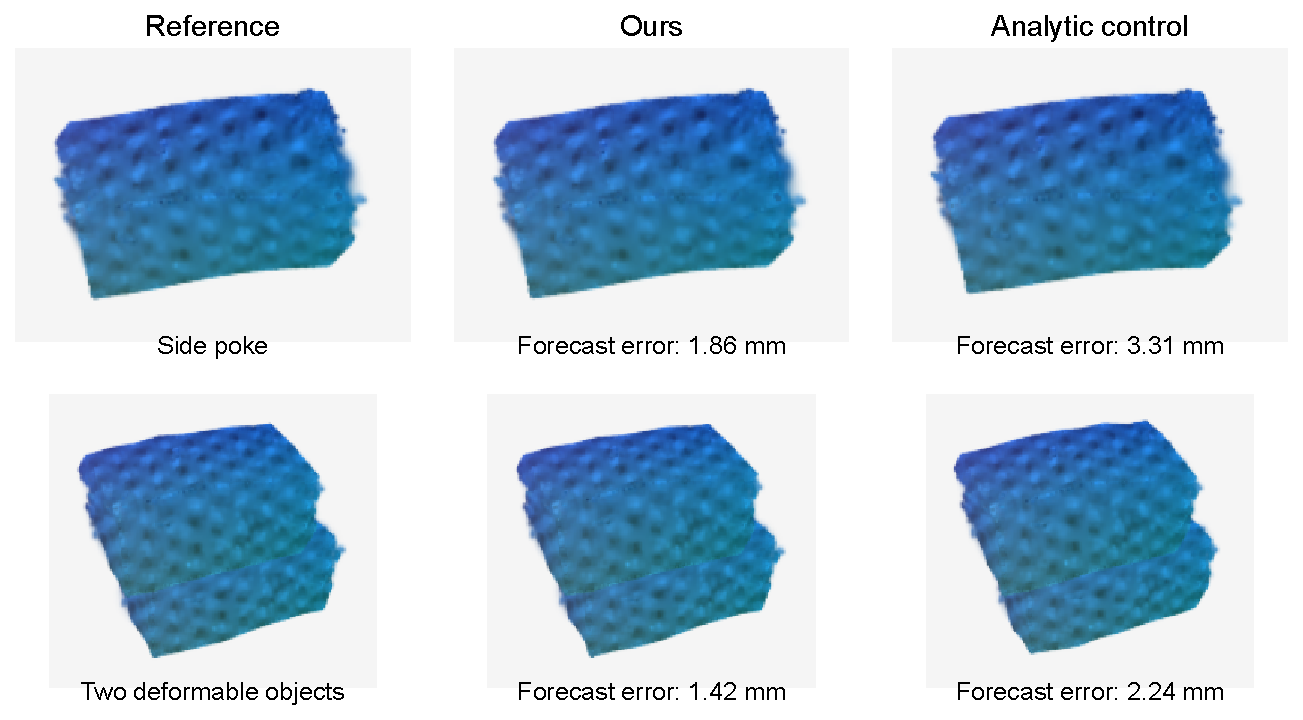
\includegraphics[width=\textwidth]{figures/solver-driven-comparisons.pdf}
\captionof{figure}{\textbf{Mechanics drives appearance under changed actions and two-object contact.} Saved predictions at the declared $0.24$\,s frame, from a withheld camera; each row uses one shared reference-derived crop. Labels report complete forecast-interval motion error, not single-frame error. No per-method alignment or deformation exaggeration is applied. The floor participates in physics but is omitted from the body-only renderer.}
\end{minipage}\end{center}



\clearpage
\paragraph{An observable action resolves an invisible scale.}
If density is unknown, multiplying mass, material energy, attachment stiffness, position-controlled target stiffness and contact penalty by the same factor leaves gravity/position-driven trajectories unchanged. We construct two hypotheses at factors one and two. Their calibration and lateral-target trajectories agree to numerical precision; a withheld-camera RGB comparison is exactly identical. A new view therefore cannot resolve this particular ambiguity. Before reading probe targets, prediction disagreement selects a calibrated force pulse over the position-controlled alternative. One RGB observation at $0.08$\,s in camera 0 selects the closer hypothesis. On a separate reversed-force action, position error falls from 1.120\,mm for the equal-prior mean to 0.448\,mm for the selected hypothesis; the other hypothesis gives 2.341\,mm. This is a constructed two-hypothesis observability test, not a calibrated posterior or a general active-policy superiority claim.

\begin{center}\begin{minipage}{\textwidth}
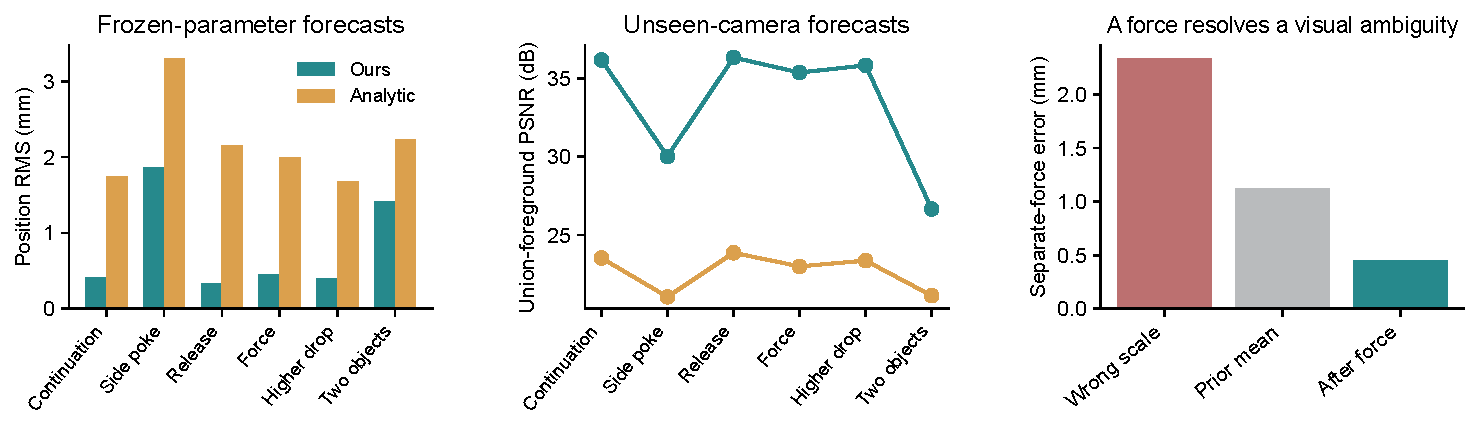
\includegraphics[width=\textwidth]{figures/solver-driven-results.pdf}
\captionof{figure}{\textbf{Physical prediction, rendering and information are tested separately.} Left and center: all six forecast scenarios. Right: a force probe resolves a mass/stiffness ambiguity that camera changes cannot resolve; evaluation uses a different force from the selected probe.}
\end{minipage}\end{center}

\paragraph{Numerical qualification and limits.}
Identity/affine transport, internal-force conservation, energy derivatives and gradients through integration pass component tests. A full rasterizer-to-material gradient check agrees with finite differences within 5.5\% at the smallest tested perturbation; larger perturbations differ by up to 20\%, reflecting the sensitivity of this piecewise rendering check. Reference refinement from $8\times4\times4$ to $16\times8\times8$ cells changes position by about 1.3\,mm; refinement to $32\times16\times16$ reduces the change to 0.76/0.61\,mm for continuation/higher drop. Halving the reference time step changes these trajectories by only 0.014/0.016\,mm. Small submillimeter differences therefore should not be interpreted as mesh-independent physical truth. The reference and predictors share a discretization family, and the learned law has a compatible invariant basis; this is a controlled coupling test rather than broad constitutive discovery. General RGB-only geometry/mass inference, unknown control histories, heterogeneous second objects, and calibrated uncertainty remain outside this qualification. Earlier public-data and six-family physical studies remain separate evidence.
\clearpage
